% Fig. 1 teaser: full-width, set under the title by main.tex (\twocolumn[{...}]).
% Design spec (2026-11-02): figures/Fig1/INDEX.md. Real OnTimeBench render and labels only; no generated imagery.
\begin{center}
\captionsetup{type=figure}
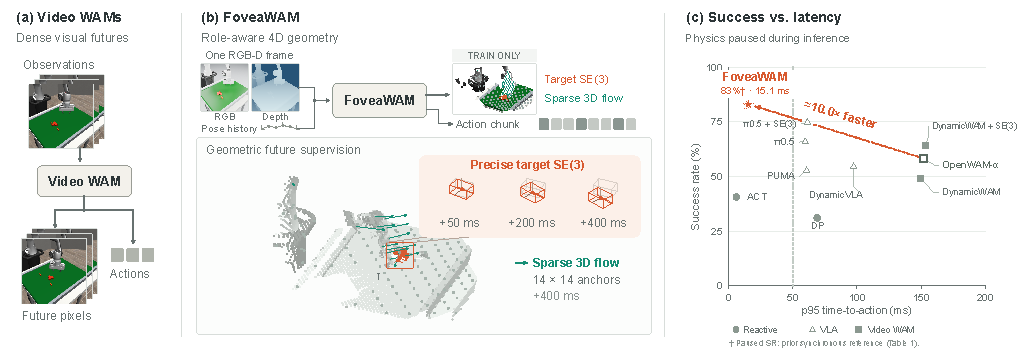
\includegraphics[width=\textwidth]{figures/Fig1/fig1.pdf}
\captionof{figure}{\textbf{\ours knows the target precisely and the rest of the scene
coarsely.} (a) A \bench frame with its training labels. The scene keeps moving while the
policy infers, so commands take effect at $\tau{+}L$ rather than at capture $\tau$. \ours
forecasts the target's metric SE(3) pose at \cfgHorizons{} horizons (axes) and the whole
scene only as a sparse 3D flow on a \cfgContextGrid{} grid (arrows; near zero on the
background). Both forecasts supervise training and are skipped at inference. (b) Success
rate on \bench against p95 time-to-action, with every method charged its own measured
latency. Dashed line: the 50\,ms control period.}
\label{fig:teaser}
\end{center}
